\documentclass[]{article}


\usepackage[utf8]{inputenc}
\usepackage{listings}
\usepackage{hyperref}
\usepackage{float}
\usepackage{graphicx}
\usepackage{subfig}
\graphicspath{ {imagenes/} }
\usepackage{xcolor}
\definecolor{RoyalBlue}{cmyk}{1, 0.50, 0, 0}
\usepackage{listings}
\lstset{language=Java,
	keywordstyle=\color{RoyalBlue},
	basicstyle=\scriptsize\ttfamily,
	commentstyle=\ttfamily\itshape\color{gray},
	stringstyle=\ttfamily,
	showstringspaces=false,
	breaklines=true,
	frameround=ffff,
	frame=single,
	rulecolor=\color{black}}



%opening
\title{práctica 1 SS: Diferentes Modelos de Simulación}
\author{José Manuel Pérez Lendínez, 26051613-l}

\begin{document}
	
	\maketitle
	
	
	\newpage
	\tableofcontents
	\newpage
	
\section{Mi Primer Modelo de Simulación de MonteCarlo}
\subsection{Descripción}
Estudiaremos un simulador que se encarga de seleccionar la mejor posición para empezar a buscar aparcamiento si quieres ir a la posición x. A la mejor posición para aparcar la denotaremos con c. Esta posición c nos indicara que no empezaremos a buscar aparcamiento hasta llegar a la plaza c. Las plazas estarán numeradas de 0 a infinito en nuestro caso y la posición x corresponderá con la plaza 100. Solo se podrá avanzar en un único sentido.
El programa tiene los siguientes parámetros:
\newline

	\textbf{./apacamiento NºRepeticiones Destino Rango\_visión Probabilidad\_aparcamiento}
\newline

El programa devuelve la posición c mencionada anteriormente y la distancia media del aparcamiento encontrado al destino.

 \subsection{Análisis con valores por defecto}
 Los valores por defectos para el software son los siguientes: 
 
 \textbf{./apacamiento 100000 100 2 0.9}
 \newline
 
 Con esto tendremos como destino la plaza 100, una visión de 2 plazas por delante nuestra y una probabilidad de ocupado en las plazas del 90\%.
 Vamos a ejecutar el programa 10 veces para comparar los resultados:
 
 \begin{table}[htbp]
 	\begin{center}
 		\begin{tabular}{|l|l|l|}
 			\hline
 			Nº ejecución & Empezar buscar(c) & Distancia media \\
 			\hline \hline
 			1 & 94&6.488250
 			 \\ \hline
 			2 & 94&6.494710
 			 \\ \hline
 			3 & 94&6.517760
 			 \\ \hline
 			4 & 94&6.499410 \\ \hline
 			5 & 94&6.502700 \\ \hline
 			6 & 93&6.493320 \\ \hline
 			7 & 94&6.489240 \\ \hline
 			8 &  94&6.447880\\ \hline
 			9 & 94&6.455970 \\ \hline
 			10 & 94&6.489890 \\ \hline
 		\end{tabular}
 		\caption{Valores por defecto.}
 		\label{tabla:sencilla}
 	\end{center}
\end{table}
 En este caso se ve como tenemos una ejecución muy parecido en todos los caso, siendo el valor para c mas elegido 94 y la distancia media muy parecida para todas las ejecuciones.
 
 Esto nos da señales de que la simulación tiene un buen método de generar el c puesto que aunque trabaje con números aleatorio siempre tiende a encontrar soluciones muy parecidas. Lo que hace que no se muy dependiente de los números aleatorios generados.
 
 \subsection{Análisis con valores extremos}
 Una buena práctica para saber si el simulador obtiene los resultados recomendables seria utilizar valores extremos de los cuales sabemos el resultado que nos daría el simulador. Un buen ejemplo sería poner la probabilidad de aparcamiento en 0. Esto haría que siempre aparcáramos en el destino(100 en nuestro caso).
 
 
 Vamos a realizar tres ejecuciones con los siguientes parametros para ver los resultados:
 \textbf{./aparcamiento 100000 100 2 0 }
 
 \begin{table}[htbp]
 	\begin{center}
 		\begin{tabular}{|l|l|l|}
 			\hline
 			Nº ejecución & Empezar buscar(c) & Distancia media \\
 			\hline \hline
 			1 & 98&0
 			\\ \hline
 			2 & 98&0
 			\\ \hline
 			3 & 98&0
 			\\ \hline
 		\end{tabular}
 		\caption{Ninguna plaza ocupada.}
 		\label{tabla:sencilla}
 	\end{center}
\end{table}

Como se ve los resultados son los esperados. Empezamos a buscar en la posición 98 puesto que tenemos una visión de dos plazas y con esto desde la 98 veríamos la plaza 100 que es nuestro destino. Y obviamente la distancia media se queda en 0 puesto que siempre aparcamos en el destino. 

Otro ejemplo que estaría bien comprobar es si le aumentamos la visión con las mismas características anteriores si c = destino - rango visión. Vamos a aumentar el rango de visión a 20 para este ejemplo: 
\textbf{./aparcamiento 100000 100 20 0 }
 
 \begin{table}[htbp]
	\begin{center}
		\begin{tabular}{|l|l|l|}
			\hline
			Nº ejecución & Empezar buscar(c) & Distancia media \\
			\hline \hline
			1 & 80&0
			\\ \hline
			2 & 80&0
			\\ \hline
			3 & 80&0
			\\ \hline
		\end{tabular}
		\caption{Ninguna plaza ocupada y mucha visión.}
		\label{tabla:sencilla}
	\end{center}
\end{table}
 
Nos da como c el número 80 por tanto nos esta dando los resultados esperados. 

Por probar algún valor extremo mas voy a probar como aumentaría la distancia en el caso de tener una porcentaje de ocupación en el aparcamiento muy elevado. Se podremos 99\%. En este caso se tendría que aumentar la distancia media y el c tendría que ser mas pequeño para empezar a buscar antes:
\textbf{./aparcamiento 100000 100 2 0.99}
 \begin{table}[htbp]
	\begin{center}
		\begin{tabular}{|l|l|l|}
			\hline
			Nº ejecución & Empezar buscar(c) & Distancia media \\
			\hline \hline
			1 & 33&68.548569
			\\ \hline
			2 & 28&68.597023
			\\ \hline
			3 & 33&68.616577
			\\ \hline
			4 & 33&68.396759
			\\ \hline
			5 & 29&68.473137
			\\ \hline
		\end{tabular}
		\caption{Ocupacion del 99\%.}
		\label{tabla:sencilla}
	\end{center}
\end{table}

Los resultados dados nos dan la razón y se ve como es necesario buscar antes y tendremos una mayor distancia media hacia el objetivo.

Por ultimo vamos a realizar el mismo ejemplo simplemente cambiando el destino para ver como se tendría que dar algo muy parecido a este ultimo, salvo que se tendría que empezar a buscar aparcamiento mas adelante si el destino lo ponemos mas lejano: 
\textbf{./aparcamiento 100000 200 2 0.99}
 \begin{table}[htbp]
	\begin{center}
		\begin{tabular}{|l|l|l|}
			\hline
			Nº ejecución & Empezar buscar(c) & Distancia media \\
			\hline \hline
			1 & 129&68.418503
			\\ \hline
			2 & 131&68.142609
			\\ \hline
			3 & 132&68.444359
			\\ \hline
			4 & 128&68.482407
			\\ \hline
			5 & 131&68.103142
			\\ \hline
		\end{tabular}
		\caption{Moviendo el destino.}
		\label{tabla:sencilla}
	\end{center}
\end{table}

Como se ve en este ejemplo simplemente se termina teniendo el valor c unas 100 plazas mas adelante, que es el valor que hemos movido el destino. 

\subsection{Análisis con cambios en los parámetros}
En este apartado vamos a analizar tres posibilidades:
\begin{enumerate}
	\item Cambio de visión: Ir aumentando la visión para ver como va cambiando el valor c.
	\item Cambio de probabilidad de aparcamiento: Ir aumentado la probabilidad de aparcamiento desde un valor bajo a uno alto para ver como aumenta la distancia de aparcamiento y el valor c disminuye.
	\item Mezcla de ambos: Mezclaremos la visión y la probabilidad de aparcamiento para ver como responde el simulador.
\end{enumerate}

\subsubsection{Cambio de visión}
Utilizaremos una visión entre 2 y 30 para ver como va mejorando. Vamos a dibujar 2 gráficas para ver la distancia media y en que posición empieza a buscar aparcamiento. Los demás parámetros se quedaran como vienen por defectos en el programa

\begin{figure}[H]
	\centering
	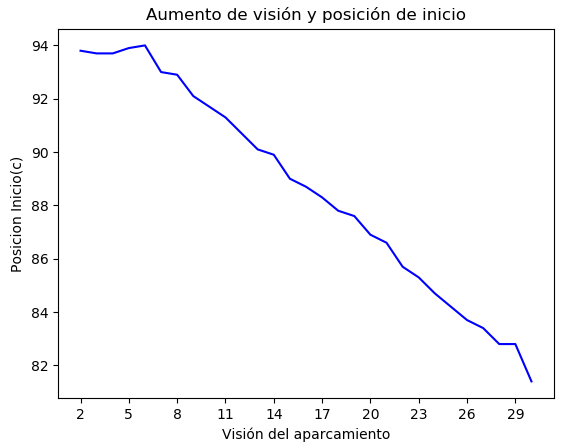
\includegraphics[width=1\linewidth]{img/screenshot011}
	\label{fig:screenshot011}
\end{figure}

Obviamente con esto se ve claramente que cuanto mas visión tendemos antes empezaremos a buscar aparcamiento, puesto que tendremos mas opciones a la vista y podremos elegir a más distancia.

\begin{figure}[H]
	\centering
	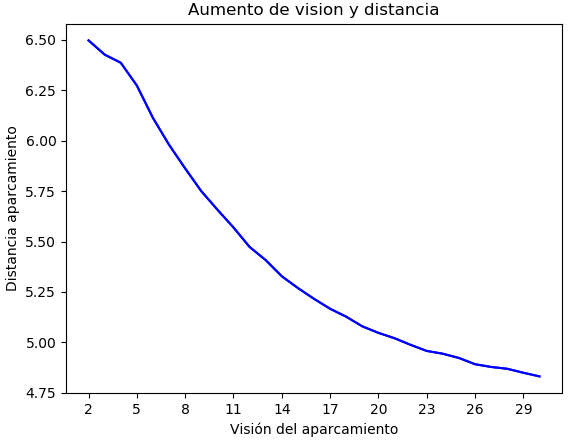
\includegraphics[width=1\linewidth]{img/screenshot008}
	\label{fig:screenshot008}
\end{figure}

En este caso el aumento de visión también afecta significativamente a la distancia de aparcamiento y se debe a que la visión nos da más opciones para aparcar. Con visión de 2 podríamos tener justo fuera del limite de nuestra visión otra plaza libre que como no tendremos en cuenta y podría ser mejor que la elegida. A más visión mas plazas de aparcamiento tendremos para elegir la mejor.





\subsubsection{Cambio de probabilidad}

Empezaremos las mediciones en 10\% de probabilidad hasta un 90\%, aumentado un 5\% cada vez.

\begin{figure}[H]
	\centering
	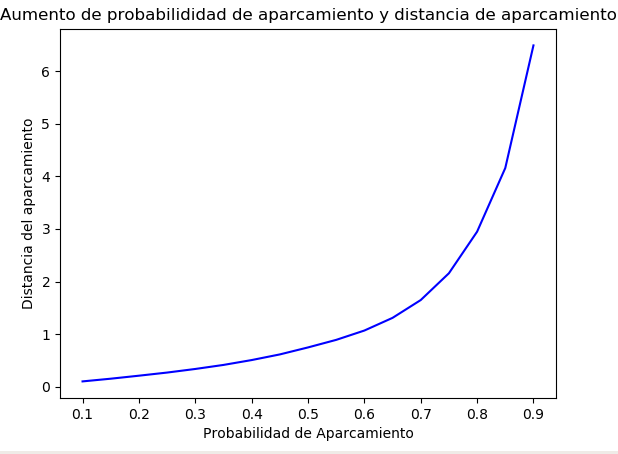
\includegraphics[width=1\linewidth]{img/screenshot014}
	\label{fig:screenshot014}
\end{figure}

En este caso se ve claramente como se obtiene menores distancias con un menor porcentaje de ocupación de las plazas. Ya que tendremos mas plazas cerca del destino. Conforme los porcentajes crecen la distancia aumenta. A partir del 50\% se ve un crecimiento mayor de dicha distancia. 

\begin{figure}[H]
	\centering
	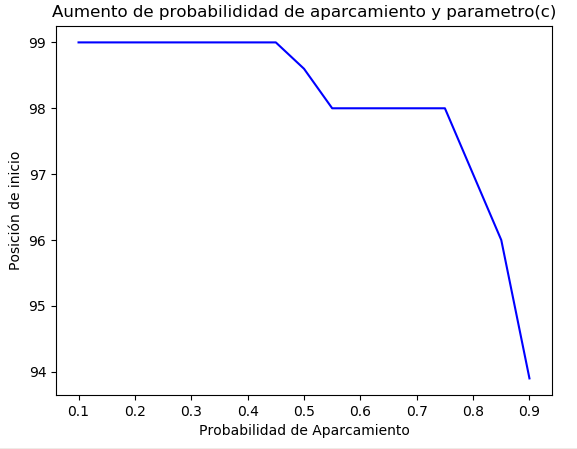
\includegraphics[width=1\linewidth]{img/screenshot013}
	\label{fig:screenshot013}
\end{figure}

En esta gráfica se ve mas claramente el escalón a partir del 50\% y como este hace que empezamos a buscar una plaza antes, aunque nos disminuye solo en una plaza. Pero si se ve más claramente como a partir del 80\% empezamos a buscar antes y como se vio en la gráfica anterior esto haría también que la distancia aumente.

Con esto podemos llegar a la conclusión de que si la probabilidad de encontrar plaza es inferior al 80\% nos sera muy fácil encontrar una cercana. El problema viene cuando el porcentaje es superior a este. Entonces si tendríamos una mayor dificultad para encontrar plazas libres y por tanto tendríamos que empezar a buscar antes.

\newpage
\subsubsection{Mezcla de visión y porcentaje de aparcamiento.}

En este caso vamos a intentar obtener unos resultados mezclando los dos parámetros para compararlos:

 \begin{table}[H]
	\begin{center}
		\resizebox{12.5cm}{!} {
			\begin{tabular}{|l|l|l|l|}
				\hline
				Porcentaje de aparcamiento & Alcance de visión & Empezar a buscar(c) & Distancia media \\
				\hline \hline
				0.7 & 2 & 98 & 1.647350
				\\ \hline
				0.7 & 10 & 94 & 1.390060
				\\ \hline
				0.7 & 15 & 91 & 1.372610
				\\ \hline
				0.7 & 20 & 90 & 1.369460
				\\ \hline
				0.75 & 20 & 89 & 1.711370
				\\ \hline
				0.8 & 15 & 91 & 2.253990	
				\\ \hline
				0.8 & 20 & 88&2.223020
				\\ \hline
			\end{tabular}
		}
		\caption{Combinación de visión y probabilidad.}
		\label{tabla:sencilla}
	\end{center}
\end{table}

Como se ve en los ejemplos anteriores lo mas importante es la probabilidad de aparcamiento. Aun poniendo valores grandes en la visión al 75\% y al 0.8\% nunca han conseguido alcanzar los valores de distancia para 70\% con visión 2. Esto nos dice que el porcentaje de aparcamiento es lo que va a decidir la distancia al final. Aunque en un mismo porcentaje de aparcamiento si obtienen mejores resultados cuanta mas alcance tenga la visión. Aunque la mejora tampoco es tan grande.

\section{Mi primer Modelo de Simulación Discreto}
\subsection{Descripción}
 
 El simulador tendrá unos radares y una cantidad de piezas de repuesto para dichos radares. Estas piezas tienen un tiempo de vida corto y puede variar entre una y otra. Para cuando una falle tendremos piezas de repuesto que podremos instalar en estos radares. Las piezas tendrán también un tiempo de reparación que tampoco sera exacto para cada pieza. El software tendrá dos formas de llamarlo :
 
 \begin{enumerate}
 	\item \textbf{./radares Nº\_piezas Nº\_simulación} : En este caso las piezas tendrían una vida útil de unos 20 días y tardarían en repararse entre 15 y 30. Cada simulación seria de 365 días
 	
 	\item \textbf{./radares Total\_radares Nº\_piezas Mínimo\_reparación Máximo\_reparación vida\_útil Días\_simulación Nº\_simulaciones} : En este caso podremos pasar los tiempos de reparación que queramos y cambiar la vida útil de las piezas. También nos da opción a simular en vez de 365 días los que nos venga mejor.
 \end{enumerate}

 
\subsection{Pruebas con distinto número de simulaciones.}
En este apartado vamos a ver como afecta el número de simulaciones a el porcentaje de tiempo sin protección de los radares. En principio vamos a comparar los valores obtenidos para 1,5,10,50,100,500 y 1000 simulaciones. Voy a mostrar en una pequeña tabla con unos cuantos valores tomados para algunos de esos número de simulaciones.
 \begin{table}[H]
	\begin{center}
		\resizebox{12.5cm}{!} {
			\begin{tabular}{|l|l|l|}
				\hline
				número de piezas & número de simulaciones & Porcentaje de desprotección \\
				\hline \hline
				5 & 1 & 34.7219
				\\ \hline
				5 & 5 & 39.0956
				\\ \hline
				5 & 10 & 30.3927
				\\ \hline
				5 & 50 & 35.3537
				\\ \hline
				5 & 100 & 36.0141
				\\ \hline
				5 & 500 & 36.9496
				\\ \hline
				5 & 1000 & 37.0519
				\\ \hline
				10 & 1 & 0.963542
				\\ \hline
				10 & 5 & 2.48001
				\\ \hline
				10 & 10 & 3.66313
				\\ \hline 
				10 & 50 & 2.17376
				\\ \hline
				10 & 100 & 2.08296
				\\ \hline
				10 & 500 & 2.19186
				\\ \hline
				10 & 1000 & 2.24074
				\\ \hline
				15 & 1 & 0
				\\ \hline
				15 & 5 & 0
				\\ \hline
				15 & 10 & 0.0861005
				\\ \hline
				15 & 50 & 0.0169635
				\\ \hline
				15 & 100 & 0.0197583
				\\ \hline
				15 & 500 & 0.0369441
				\\ \hline
				15 & 1000 & 0.0203786
				\\ \hline
				
			\end{tabular}
		}
		\caption{Combinación de visión y probabilidad.}
		\label{tabla:sencilla}
	\end{center}
\end{table}
Como se ve en la tabla a partir de 15 piezas de reserva obtenemos porcentajes por debajo de 1\% para todos los números de simulaciones realizados.

Con un número de simulaciones bajas tenemos el problema de que los resultados no son muy representativos puesto que cambian mucho los valores de una ejecucion a otra. La gráfica siguiente muestra las diferencias obtenidas para tres ejecuciones de 10 simulaciones.

\begin{figure}[H]
	\centering
	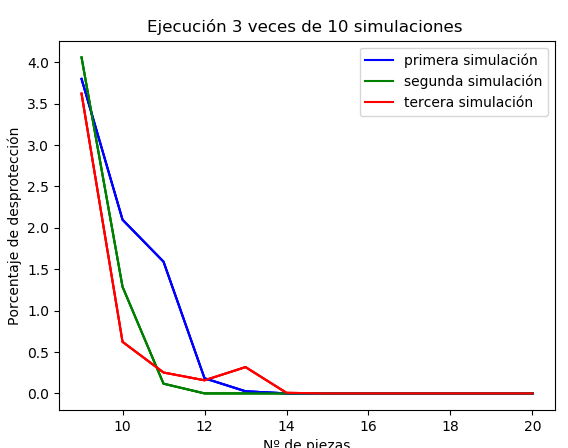
\includegraphics[width=1\linewidth]{img/screenshot0016}
	\label{fig:screenshot0016}
\end{figure}

Como se ve obtenemos distintos valores y no son muy parecidas. En cambio cuando tenemos número de simulaciones mayares tienden a parecerse mucho mas como en el siguiente ejemplo.

\begin{figure}[H]
	\centering
	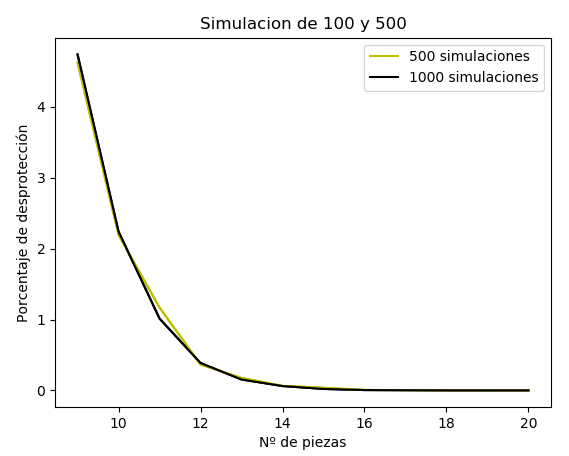
\includegraphics[width=1\linewidth]{img/screenshot0017}
	\label{fig:screenshot0017}
\end{figure}
Como se ve en la gráfica anterior comparamos la simulación con 500 y 1000 repeticiones, viendo que estas ya si son mas cercanas la una a la otra. Esto nos dice que para tener resultados mas exactos y que no varíen tanto tendremos que usar valores mas altos en el número de simulaciones. Vamos a ver la tabla para un número de 1000 simulaciones y analizarla.

 \begin{table}[H]
	\begin{center}
		\resizebox{12.5cm}{!} {
			\begin{tabular}{|l|l|l|}
				\hline
				número de piezas & número de simulaciones & Porcentaje de desprotección \\
				\hline \hline
				10 & 1000 & 0.971745
				\\ \hline
				11 & 1000 & 0.971745
				\\ \hline
				12 & 1000 & 0.43975
				\\ \hline
				13 & 1000 & 0.155862
				\\ \hline
				14 & 1000 & 0.0644814
				\\ \hline
			\end{tabular}
		}
		\caption{Combinación de visión y probabilidad.}
		\label{tabla:sencilla}
	\end{center}
\end{table}

Con esto se ve claramente que pasamos la barrera del 1\% con 11 o mas piezas. Pero en el caso de 11 se quedaría muy justo y en otros caso nos podría dar valores un poquito mayores que el 1\%, por tanto elegiríamos 12 o mas piezas para cumplirlo siempre. 

\subsection{Pruebas con vida útil}
En este apartado vamos a ver como cambia el porcentaje de desprotección cambiando tanto la vida útil como el tiempo de reparación para un ejemplo con 1000 simulaciones.

\begin{figure}[H]
	\centering
	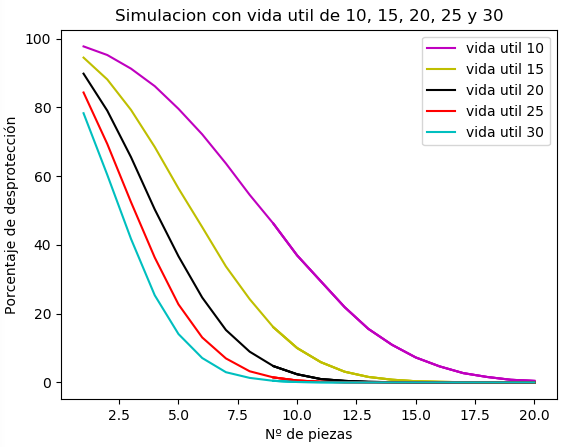
\includegraphics[width=1\linewidth]{img/screenshot0018}
	\label{fig:screenshot0018}
\end{figure}

Los resultados son los esperados, teniendo que con una vida útil mayor se consiguen mejores resultados al fallar menos la piezas. Estos nos dice que si se consiguiera mejorar la vida útil en 10 días, consiguiendo una vida útil de 30 días, conseguiríamos llegar por debajo del 1\% con solo 9 dispositivos. De este dato también sacamos que con 20 dispositivos tendríamos en todos los caso de vida útil estudiados un porcentaje de desprotección inferior al 1\%.
\newpage
\subsection{Pruebas con la tasa de arreglo.}
En este ejemplo vamos a estudiar como actua el sistema con tasas de arreglo distintas. 
\begin{figure}[H]
	\centering
	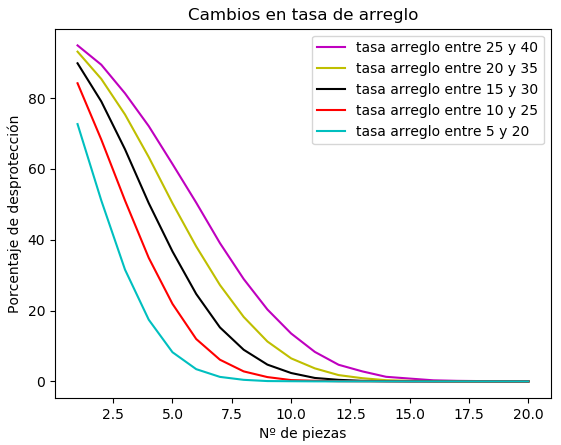
\includegraphics[width=1\linewidth]{img/screenshot0019}
	\caption{}
	\label{fig:screenshot0019}
\end{figure}

En el gráfico anterior podemos ver varias cosas importantes. Una de ellas es que simplemente mejorando el intervalo de la tasas de arreglo en 5 días obtendríamos el porcentaje inferior a 1\% con 10 piezas. Por lo tanto una buena mejora en las tasas de arreglo supondría que nos hicieran falta unos 2 repuestos menos como mínimo. Otra cosa que también nos deja claro este gráfico es que llegado a los 16 repuestos la tasa de arreglo no son tan importantes para alcanzar nuestro objetivos, siempre y cuando las tasas de arreglo no superen los 40 días.
\newpage
\section{Mi primer Modelo de Simulación Continuo}
\subsection{Descripción}
Vamos a estudiar un simulador que se encarga de simular el crecimiento de dos especies de peces. La especie de peces pequeños y la especie de peces grande. Los grandes necesitaran alimentarse de peces pequeños para sobrevivir y que su número no se reduzca. En cambio se limita el número de peces pequeños para no poder tener un número de peces ilimitado. Este simulador nos servirá para ver que cuando se equilibra la población de estas dos especies y viven juntas en el lago sin llegar a extremos que puedan hacer que se extingan.
\subsection{Búsqueda de estabilidad.}
Vamos a buscar la estabilidad de la población para conseguir tener un número de peces grandes y pequeños que se mantenga casi igual a lo largo de todos los días. Para esto necesitaremos fijar un número de peces grandes y pequeños para iniciar el programa. Después de unas cuantas pruebas he conseguido una población estable utilizados 2000 peces pequeños y 15 peces grandes. Con estos resultados obtenemos la siguiente gráfica:
\begin{figure}[H]
	\centering
	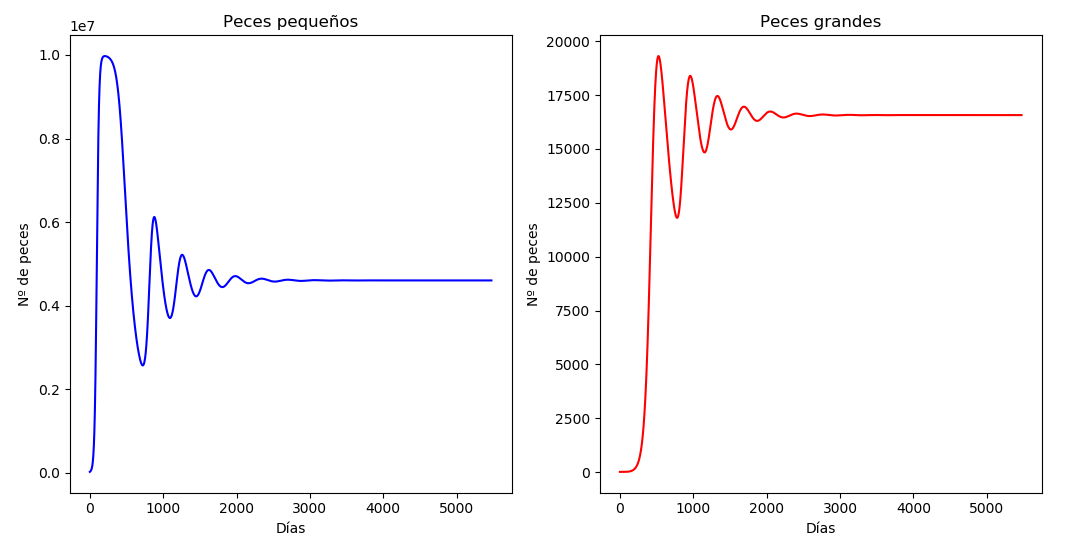
\includegraphics[width=1\linewidth]{img/screenshot0024}
	\caption{}
	\label{fig:screenshot0024}
\end{figure}
Como se ven en estas gráficas cerca de los tres mil días se consigue la estabilidad y no se dan mas cambios teniendo un total de 4,5 millones de peces pequeños y unos 16500 peces grandes. 
Vamos a analizar una gráfica que nos mostrara mas claramente en que valores se vuelve estable la población.
\begin{figure}[H]
	\centering
	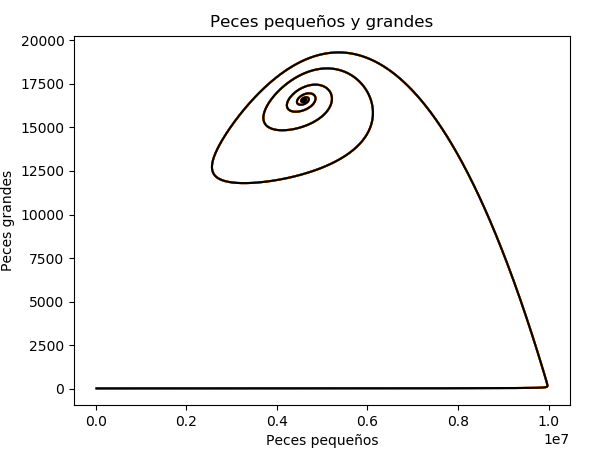
\includegraphics[width=0.7\linewidth]{img/screenshot0021}
	\label{fig:screenshot0021}
\end{figure}

En esta gráfica se ve como empieza a crecer la población y entra en un ciclo que se va reduciendo hasta llegar al los valores de estabilidad dados en las gráficas anteriores.

\subsection{Ejemplo de pesca}
Para probar los cambios añadidos al código una opción que permiten tener campañas de pesca. Vamos a realizar una campaña de pesca justo cuando lleguemos a la mitad de los días simulados. En nuestro caso simularemos siempre 15 años. La campaña de pesca que realizaremos sera del 50\% de los peces grandes como se dice en el pdf de la práctica.

\begin{figure}[H]
	\centering
	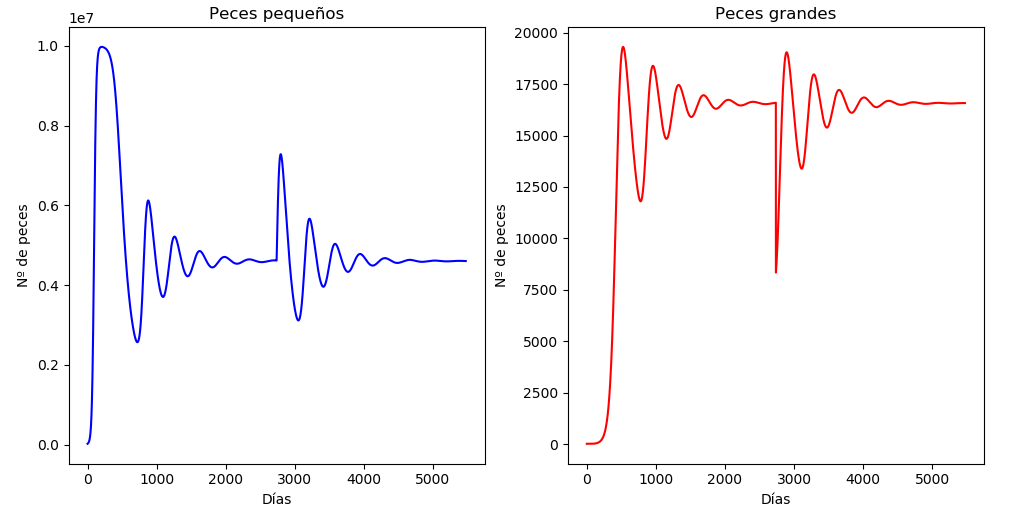
\includegraphics[width=1\linewidth]{img/screenshot0030}
	\caption{}
	\label{fig:screenshot0030}
\end{figure}
Como se ve al llegar al 50\% de los días de simulación se capturan el 50 por ciento de los ejemplares de peces grandes lo que hace que estos tengan un pico que baje y el efecto contrario en los peces pequeños. Los peces pequeños al tener menos depredadores crecen. Esto se va igualando nuevamente puesto que los depredadores que quedan tienen mas alimento y empiezan a crecer nueva mente hasta equilibrarse como al principio de la simulación, justo antes de la campaña de pesca. 

En la siguiente gráfica se puede ver como la población llega un momento en la que se estabiliza. Después debido a la campaña de pesca salimos de la zona donde estabilizamos y se crea un nuevo ciclo que vuelve a llevar a la zona donde se consiguió la población estable. Esto se da entorno a los 4,5 millones de peces pequeños y unos 16500 peces grandes.
\begin{figure}[H]
	\centering
	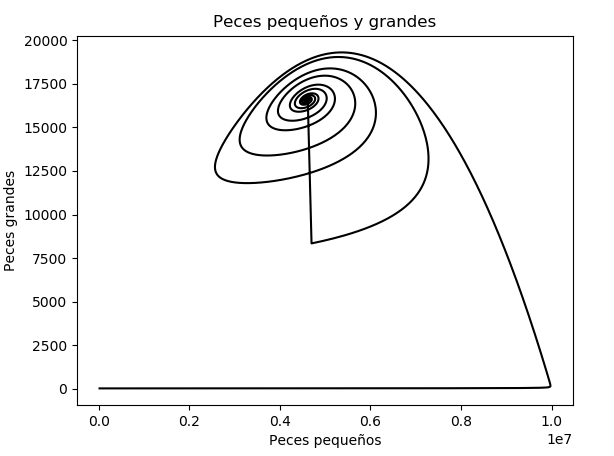
\includegraphics[width=0.7\linewidth]{img/screenshot0031}
	\caption{}
	\label{fig:screenshot0031}
\end{figure}




\subsection{Estudio de pesca.}
Al tener una población que se estabiliza podemos intentar realizar una política de pesa para obtener el mayor número de peces posibles sin que la población de peces se desequilibre o desaparezca. Para esto tendremos que ver distintas formas de realizar la pesca y quedarnos con el número de peces obtenido con estas formas.

 Vamos a tener en cuenta que nuestros peces se reproducen de igual manera durante todo el año y no tienen épocas especificas de reproducción. Esto me dice que lo mas probable seria una política de pesca en la que se pesque cada pocos dias y un porcentaje pequeño de peces. Si esto no fuera así tendríamos que probar otras políticas de pesca que tuvieran mas en cuenta cuando se reproducen estos peces. De todos modos vamos afrontar esto con cuatro formas de pesca para cubrir todas las opciones:
\newpage
\begin{enumerate}
	\item \textbf{Pesca semanal}: Tendremos una pesca a la semana, con un porcentaje bajo de la población. 
	\item \textbf{Pesca mensual}: Una pesca cada 30 días en la que se pesque un porcentaje un poco mayor de la población. 
	\item \textbf{Pesca trimestral}: En este caso pescaremos cada 60 días y subiremos un poquito mas la cantidad de peces a pescar.
	\item \textbf{Pesca semestral}: Pescaremos cada 180 días y con un porcentaje aun mayor de la población.
\end{enumerate}

Para obtener los porcentajes de cada ejemplo del apartado anterior ejecutare el programa con varios valores distintos y me quedare el mejor para cada tipo de pesca. Obviamente las campañas de pesca no pueden ser muy agresivas ya que sino capturaríamos todas la población y se desequilibraría, de forma que la población despareciera. Para esto la simulación la realizaremos para un total de 15 años como las anteriores.

Los porcentajes elegidos para cada tipo de pesca después de las pruebas realizadas son los siguientes porcentajes de la población (Marcados en negro):

\begin{enumerate}
	\item \textbf{Pesca semanal}:
	\begin{table}[H]
		\begin{center}
			\begin{tabular}{|l|l|}
				\hline
				Porcentaje pesca & Total pescado\\
				\hline \hline
				0.05 & 424731
				\\ \hline
				0.06 & 491976
				\\ \hline
				\textbf{0.07} & \textbf{560092}
				\\ \hline
				0.08 & 527187
				\\ \hline
				0.09 & 468843
				\\ \hline
			\end{tabular}
			\label{tabla:sencilla}
		\end{center}
	\end{table}
	\item \textbf{Pesca mensual}: 
	\begin{table}[H]
		\begin{center}
			\begin{tabular}{|l|l|}
				\hline
				Porcentaje pesca & Total pescado\\
				\hline \hline
				0.2 & 494195
				\\ \hline
				0.25 & 549716
				\\ \hline
				\textbf{0.3} & \textbf{555694}
				\\ \hline
				0.35 & 497590
				\\ \hline
				0.4 & 357525
				\\ \hline
			\end{tabular}
			\label{tabla:sencilla}
		\end{center}
	\end{table}
	\item \textbf{Pesca trimestral}:
	\begin{table}[H]
		\begin{center}
			\begin{tabular}{|l|l|}
				\hline
				Porcentaje pesca & Total pescado\\
				\hline \hline
				0.55 & 509228
				\\ \hline
				0.6 & 527822
				\\ \hline
				\textbf{0.65} & \textbf{529367}
				\\ \hline
				0.70 & 504574
				\\ \hline
				0.75 & 436986
				\\ \hline
			\end{tabular}
			\label{tabla:sencilla}
		\end{center}
	\end{table}
	\item \textbf{Pesca semestral}:
	
	\begin{table}[H]
		\begin{center}
			\begin{tabular}{|l|l|}
				\hline
				Porcentaje pesca & Total pescado\\
				\hline \hline
				0.75 & 398577
				\\ \hline
				0.8 & 422392
				\\ \hline
				\textbf{0.85} & \textbf{439416}
				\\ \hline
				0.9 & 436237
				\\ \hline
				0.95 & 343561
				\\ \hline
			\end{tabular}
			\label{tabla:sencilla}
		\end{center}
	\end{table}
\end{enumerate}


Vamos a realizar un gráfico de barras para comparar cual es el mejor modelo de pesca:
\begin{figure}[H]
	\centering
	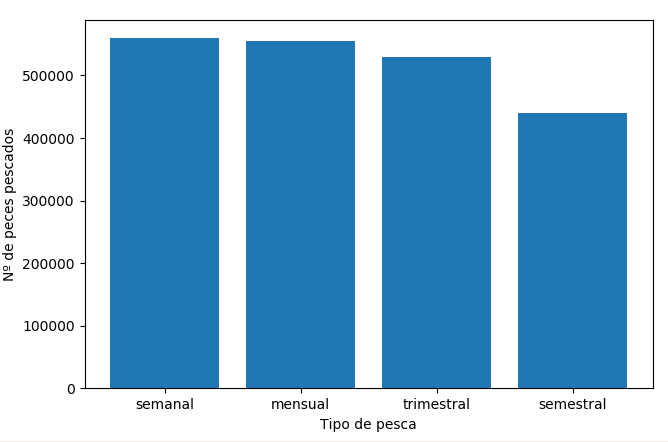
\includegraphics[width=1\linewidth]{img/screenshot0025}
	\label{fig:screenshot0025}
\end{figure}
\newpage
Como se ve en el histograma tenemos prácticamente la misma cantidad de peces con el método semanal y mensual. Quedando por detrás el trimestral muy cerca y el semestral el peor.


Con esto podemos darnos cuenta de que la forma de pescar tampoco es lo más importante. Es más importante saber elegir el porcentaje de peces que tendremos que pescar según nuestra frecuencia de pesca. Por ejemplo en el semanal pescamos un 7\% de la población total mientras que en el mensual pescamos el 30\%. Esto también se da porque el simulador no tiene en cuenta problemas externos que pudieran hacer que se extinguiera la población de peces por alguna enfermedad o por falta de comida debido a algún fenómeno que no podemos controlar. En esos caso seria mejor pescar semanalmente puesto que tenemos siempre una población mas alta durante todo el año que si pescáramos trimestralmente por ejemplo.


Vamos a mostrar las gráficas de la pesca semanal y semestral para ver como evoluciona la población en los extremos de nuestros métodos de pesca.


\begin{enumerate}
	\item \textbf{Pesca semanal:}
	\begin{figure}[H]
		\centering
		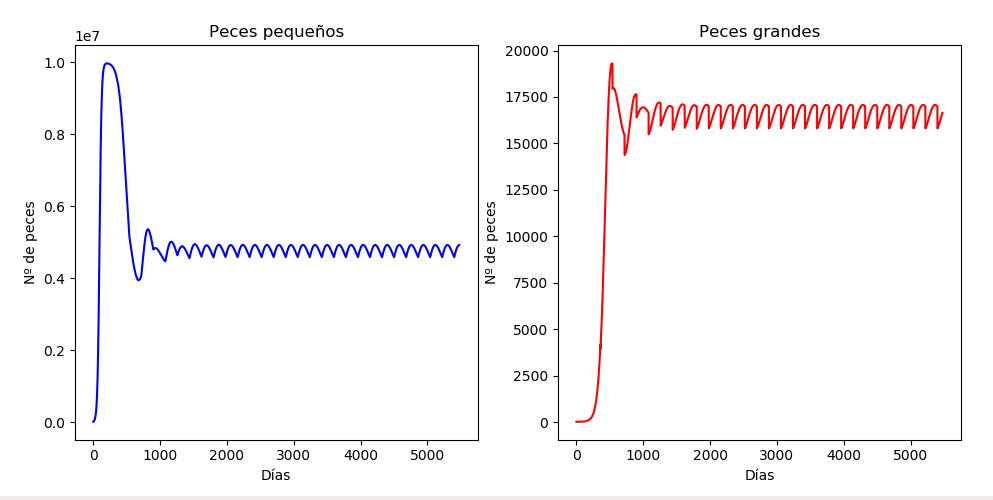
\includegraphics[width=1\linewidth]{img/screenshot0026}
		\label{fig:screenshot0026}
	\end{figure}
	Como se ve en la pesca semanal tenemos una población mas o menos igualada durante todo el tiempo de ejecucion sin grandes picos que nos dejaran con pocos peces o demasiados como para correr el riesgo de que se llegue a extremos donde las condiciones no sean validad y se pierda toda la población.
	Una vez visto esto la comparación entre peces grandes y pequeñas nos saldrá muy bien definida y sin muchos saltos.
	\begin{figure}[H]
		\centering
		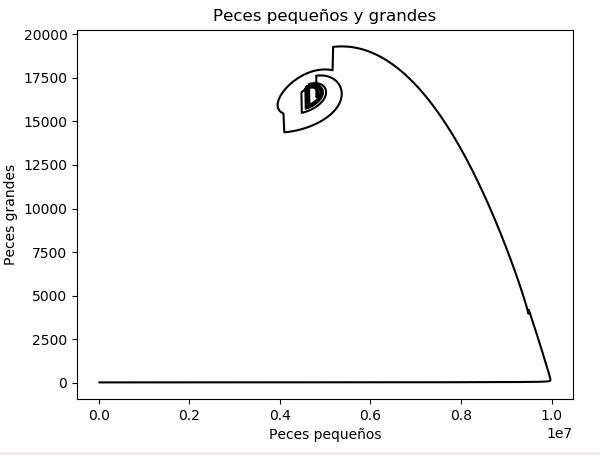
\includegraphics[width=0.7\linewidth]{img/screenshot0027}
		\label{fig:screenshot0027}
	\end{figure}

	

	\item \textbf{Pesca semestral:}
	\begin{figure}[H]
		\centering
		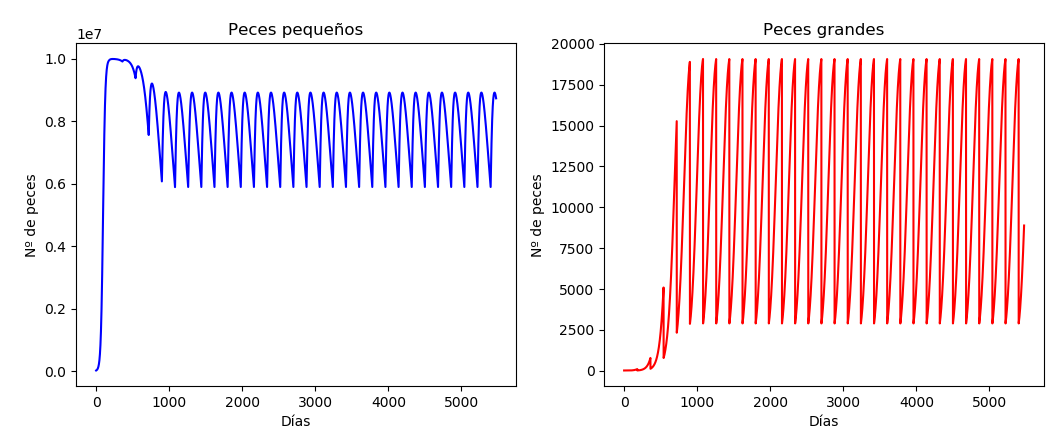
\includegraphics[width=1\linewidth]{img/screenshot0028}
		\label{fig:screenshot0028}
	\end{figure}
	En este caso estamos viendo como los peces grandes llegan a extremos bastantes mas marcados que en el método anterior. Esto se debe a que al pescar el 85\% de los peces grandes estos tienden a estar mas cerca de reducir el número total de estos peces. Esto nos podría dar problemas si después de una pesca se diera una enfermedad en los peces grandes que los podría llevar a la extinción antes de volver a recuperarse (aunque nuestro simulador no tenga estas cosas en cuenta). También vemos que al tener una cantidad promedia de peces grandes menor, los peces pequeños aumentan sus números mas que en el caso anterior. 
	\newpage
	Obviamente con estos datos veremos que la gráfica que muestra las proporciones de peces grandes y pequeños sera mas difícil de analizar que la anterior, puesto que tenemos una mayor variación en el número de peces.
	
	\begin{figure}[H]
		\centering
		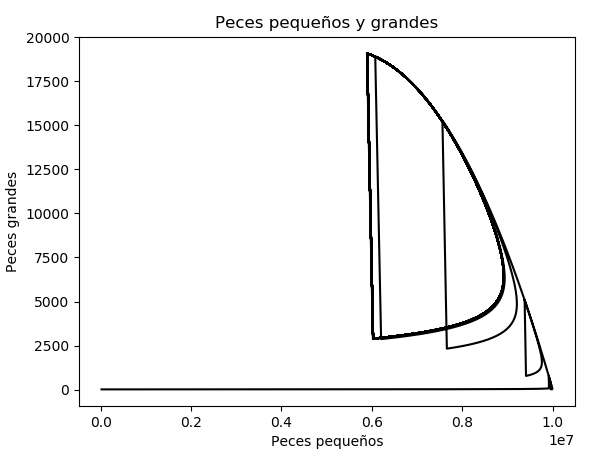
\includegraphics[width=0.7\linewidth]{img/screenshot0029}
		\label{fig:screenshot0029}
	\end{figure}
	En este caso el ciclo que representa a los peces grandes respecto a los pequeños es mas grande por la variación explicada anteriormente y esto hace esta gráfica mas difícil de analizar que la anterior.
\end{enumerate}










 
 
	
\end{document}
